\documentclass[UTF8,11pt]{ctexart}
\usepackage[a4paper,margin=22mm]{geometry}
\usepackage{amsmath,amssymb,bm,graphicx,adjustbox,fvextra,longtable,array}
\xeCJKDeclareCharClass{CJK}{"2160 -> "217F, "2460 -> "249B, "2200 -> "22FF}
\newcommand{\fitmath}[1]{\begin{adjustbox}{max width=\linewidth}$\displaystyle #1$\end{adjustbox}}
\setlength{\parindent}{0pt}\setlength{\parskip}{.65em}\renewcommand{\arraystretch}{1.3}
\sloppy\allowdisplaybreaks
\begin{document}
\section*{2015 年计算机统考 408 · 真题及解析}
\subsection*{2015 年全国硕士研究生入学统一考试}

\subsection*{计算机科学与技术学科联考计算机学科专业基础综合试题}

\subsection*{一、单项选择题：第1～40小题，每小题2分，共80分。下列每题给出的四个选项中，只有一个选项最符合试题要求。}

1．已知程序如下：


\begin{Verbatim}[breaklines,breakanywhere,fontsize=\small]
int S(int n)
{  return (n<=0)?0:s(n-1)+n;}
void main()
{  cout<< S(1); }
\end{Verbatim}

程序运行时使用栈来保存调用过程的信息，自栈底到栈顶保存的信息依次对应的是\_\_\_\_\_\_。A．main()→S(1)→S(0)　B．S(0)→S(1)→main()　B．main()→S(0)→S(1)　D．S(1)→S(0)→main()


2．先序序列为 a,b,c,d 的不同二叉树的个数是\_\_\_\_\_\_。A．13　B．14　C．15　D．16


3．下列选项给出的是从根分别到达两个叶结点路径上的权值序列，能属于同一棵哈夫曼树的是\_\_\_\_\_\_。A．24,10,5 和 24,10,7　B．24,10,5 和 24,12,7　C．24,10,10 和 24,14,11　D．24,10,5 和 24,14,6


4．现有一棵无重复关键字的平衡二叉树（AVL树），对其进行中序遍历可得到一个降序序列。下列关于该平衡二叉树的叙述中，正确的是\_\_\_\_\_\_。A．根结点的度一定为2　B．树中最小元素一定是叶结点　C．最后插入的元素一定是叶结点　D．树中最大元素一定是无左子树


5．设有向图 \(\displaystyle G=(V,\allowbreak E)\)，顶点集 \(\displaystyle V=\{V_0,\allowbreak V_1,\allowbreak V_2,\allowbreak V_3\}\)，边集 \(\displaystyle E=\{\langle v_0,\allowbreak v_1\rangle,\allowbreak \langle v_0,\allowbreak v_2\rangle,\allowbreak \langle v_0,\allowbreak v_3\rangle,\allowbreak \langle v_1,\allowbreak v_3\rangle\}\)。若从顶点 \(\displaystyle V_0\) 开始对图进行深度优先遍历，则可能得到的不同遍历序列个数是\_\_\_\_\_\_。A．2　B．3　C．4　D．5


6．求下面带权图的最小（代价）生成树时，可能是克鲁斯卡（Kruskal）算法第2次选中但不是普里姆（Prim）算法（从 \(\displaystyle V_4\) 开始）第2次选中的边是\_\_\_\_\_\_。A．\(\displaystyle (V_1,\allowbreak V_3)\)　B．\(\displaystyle (V_1,\allowbreak V_4)\)　C．\(\displaystyle (V_2,\allowbreak V_3)\)　D．\(\displaystyle (V_3,\allowbreak V_4)\)


\begin{center}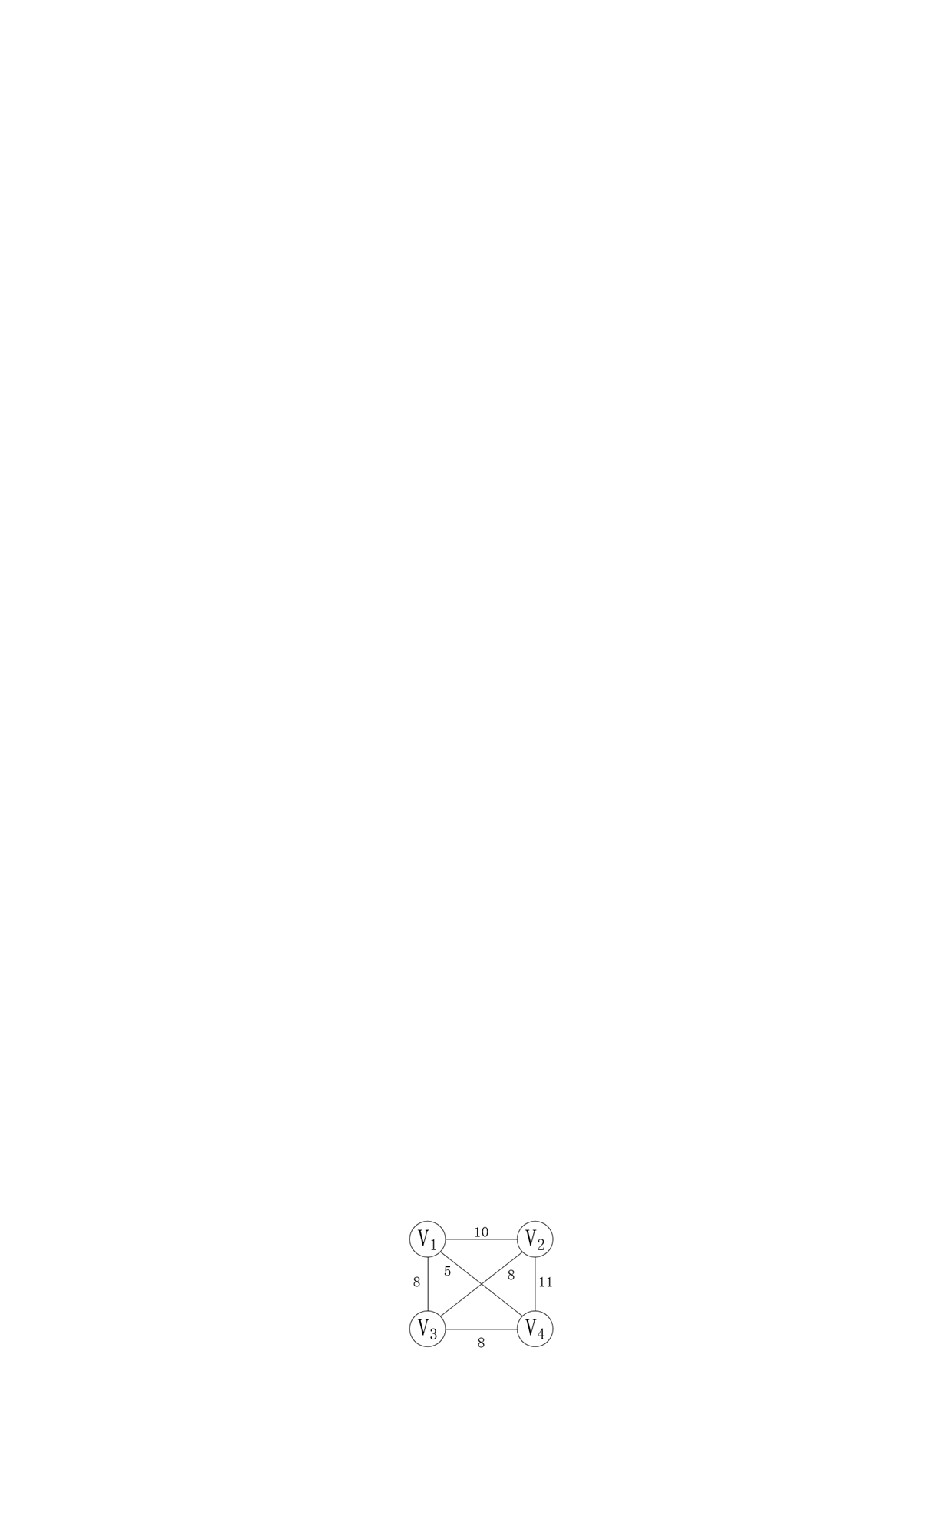
\includegraphics[width=.65\linewidth,height=.4\textheight,keepaspectratio]{../assets/figures/2015-complete-p001-b011.pdf}\end{center}

7．下列选项中，不能构成折半查找中关键字比较序列的是\_\_\_\_\_\_。A．500,200,450,180　B．500,450,200,180


7．（续）C．180,500,200,450　D．180,200,500,450


8．已知字符串 S 为“abaabaabacacaabaabcc”，模式串 t 为“abaabc”。采用 KMP 算法进行匹配，第一次出现“失配”（s[i]≠t[j]）时，i=j=5，则下次开始匹配时，i 和 j 的值分别是\_\_\_\_\_\_。A．i=1,j=0　B．i=5,j=0　C．i=5,j=2　D．i=6,j=2


9．下列排序算法中，元素的移动次数与关键字的初始排列次序无关的是\_\_\_\_\_\_。A．直接插入排序　B．起泡排序　C．基数排序　D．快速排序


10．已知小根堆为8,15,10,21,34,16,12，删除关键字8之后需重建堆，在此过程中，关键字之间的比较次数是\_\_\_\_\_\_。A．1　B．2　C．3　D．4


11．希尔排序的组内排序采用的是\_\_\_\_\_\_。A．直接插入排序　B．折半插入排序　C．快速排序　D．归并排序


12．计算机硬件能够直接执行的是\_\_\_\_\_\_。Ⅰ．机器语言程序　Ⅱ．汇编语言程序　Ⅲ．硬件描述语言程序。A．仅Ⅰ　B．仅Ⅰ、Ⅱ　C．仅Ⅰ、Ⅲ　D．Ⅰ、Ⅱ、Ⅲ


13．由3个“1”和5个“0”组成的8位二进制补码，能表示的最小整数是\_\_\_\_\_\_。A．-126　B．-125　C．-32　D．-3


14．下列有关浮点数加减运算的叙述中，正确的是\_\_\_\_\_\_。Ⅰ．对阶操作不会引起阶码上溢或下溢；Ⅱ．右规和尾数舍入都可能引起阶码上溢；Ⅲ．左规时可能引起阶码下溢；Ⅳ．尾数溢出时结果不一定溢出。A．仅Ⅱ、Ⅲ　B．仅Ⅰ、Ⅱ、Ⅳ　C．仅Ⅰ、Ⅲ、Ⅳ　D．Ⅰ、Ⅱ、Ⅲ、Ⅳ


15．假定主存地址为32位，按字节编址，主存和 Cache 之间采用直接映射方式，主存块大小为4个字，每字32位，采用回写（Write Back）方式，则能存放4K字数据的 Cache 的总容量的位数至少是\_\_\_\_\_\_。A．146k　B．147K　C．148K　D．158K


16．假定编译器将赋值语句“x=x+3;”转换为指令“add xaddr, 3”，其中 xaddr 是 x 对应的存储单元地址。若执行该指令的计算机采用页式虚拟存储管理方式，并配有相应的 TLB，且 Cache 使用直写（Write Through）方式，则完成该指令功能需要访问主存的次数至少是\_\_\_\_\_\_。A．0　B．1　C．2　D．3


17．下列存储器中，在工作期间需要周期性刷新的是\_\_\_\_\_\_。A．SRAM　B．SDRAM　C．ROM　D．FLASH


18．某计算机使用4体交叉编址存储器，假定在存储器总线上出现的主存地址（十进制）序列为8005，8006，8007，8008，8001，8002，8003，8004，8000，则可能发生访存冲突的地址对是\_\_\_\_\_\_。A．8004和8008　B．8002和8007　C．8001和8008　D．8000和8004


19．下列有关总线定时的叙述中，错误的是\_\_\_\_\_\_。A．异步通信方式中，全互锁协议最慢　B．异步通信方式中，非互锁协议的可靠性最差　C．同步通信方式中，同步时钟信号可由各设备提供　D．半同步通信方式中，握手信号的采样由同步时钟控制


20．若磁盘转速为7200转/分，平均寻道时间为8ms，每个磁道包含1000个扇区，则访问一个扇区的平均存取时间大约是\_\_\_\_\_\_。A．8.1ms　B．12.2ms　C．16.3ms　D．20.5ms


21．在采用中断 I/O 方式控制打印输出的情况下，CPU 和打印控制接口中的 I/O 端口之间交换的信息不可能是\_\_\_\_\_\_。A．打印字符　B．主存地址　C．设备状态　D．控制命令


22．内部异常（内中断）可分为故障（fault）、陷阱（trap）和终止（abort）三类。下列有关内部异常的叙述中，错误的是\_\_\_\_\_\_。A．内部异常的产生与当前执行指令相关　B．内部异常的检测由 CPU 内部逻辑实现　C．内部异常的响应发生在指令执行过程中　D．内部异常处理后返回到发生异常的指令继续执行


23．处理外部中断时，应该由操作系统保存的是\_\_\_\_\_\_。A．程序计数器（PC）的内容　B．通用寄存器的内容　C．块表（TLB）中的内容　D．Cache 中的内容


24．假定下列指令已装入指令寄存器，则执行时不可能导致 CPU 从用户态变为内核态（系统态）的是\_\_\_\_\_\_。A．DIV R0,R1；(R0)/(R1)→R0　B．INT n；产生软中断　C．NOT R0；寄存器 R0 的内容取非　D．MOV R0,addr；把地址 addr 处的内存数据放入寄存器 R0 中


25．下列选项中，会导致进程从执行态变为就绪态的事件是\_\_\_\_\_\_。A．执行 P（wait）操作　B．申请内存失败　C．启动 I/O 设备　D．被高优先级进程抢占


26．若系统 \(\displaystyle S_1\) 采用死锁避免方法，\(\displaystyle S_2\) 采用死锁检测方法。下列叙述中，正确的是\_\_\_\_\_\_。Ⅰ．\(\displaystyle S_1\) 会限制用户申请资源的顺序，而 \(\displaystyle S_2\) 不会；Ⅱ．\(\displaystyle S_1\) 需要进程运行所需资源总量信息，而 \(\displaystyle S_2\) 不需要；Ⅲ．\(\displaystyle S_1\) 不会给可能导致死锁的进程分配资源，而 \(\displaystyle S_2\) 会。A．仅Ⅰ、Ⅱ　B．仅Ⅱ、Ⅲ　C．仅Ⅰ、Ⅲ　D．Ⅰ、Ⅱ、Ⅲ


27．系统为某进程分配了4个页框，该进程已访问的页号序列为2,0,2,9,3,4,2,8,2,4,8,4,5。若进程要访问的下一页的页号为7，依据 LRU 算法，应淘汰页的页号是\_\_\_\_\_\_。A．2　B．3　C．4　D．8


28．在系统内存中设置磁盘缓冲区的主要目的是\_\_\_\_\_\_。A．减少磁盘 I/O 次数　B．减少平均寻道时间　C．提高磁盘数据可靠性　D．实现设备无关性


29．在文件的索引节点中存放直接索引指针10个，一级和二级索引指针各1个。磁盘块大小为1KB，每个索引指针占4个字节。若某文件的索引节点已在内存中，则把该文件偏移量（按字节编址）为1234和307400处所在的磁盘块读入内存，需访问的磁盘块个数分别是\_\_\_\_\_\_。A．1,2　B．1,3　C．2,3　D．2,4


30．在请求分页系统中，页面分配策略与页面置换策略不能组合使用的是\_\_\_\_\_\_。A．可变分配，全局置换　B．可变分配，局部置换


30．（续）C．固定分配，全局置换　D．固定分配，局部置换


31．文件系统用位图法表示磁盘空间的分配情况，位图存于磁盘的32～127号块中，每个盘块占1024个字节，盘块和块内字节均从0开始编号。假设要释放的盘块号为409612，则位图中要修改的位所在的盘块号和块内字节序号分别是\_\_\_\_\_\_。A．81、1　B．81、2　C．82、1　D．82、2


32．某硬盘有200个磁道（最外侧磁道号为0），磁道访问请求序列为：130,42,180,15,199，当前磁头位于第58号磁道并从外侧向内侧移动。按照 SCAN 调度方法处理完上述请求后，磁头移过的磁道数是\_\_\_\_\_\_。A．208　B．287　C．325　D．382


33．通过 POP3 协议接收邮件时，使用的传输层服务类型是\_\_\_\_\_\_。A．无连接不可靠的数据传输服务　B．无连接可靠的数据传输服务　C．有连接不可靠的数据传输服务　D．有链接可靠的数据传输服务


34．使用两种编码方案对比特流01100111进行编码的结果如下图所示，编码1和编码2分别是\_\_\_\_\_\_。


\begin{center}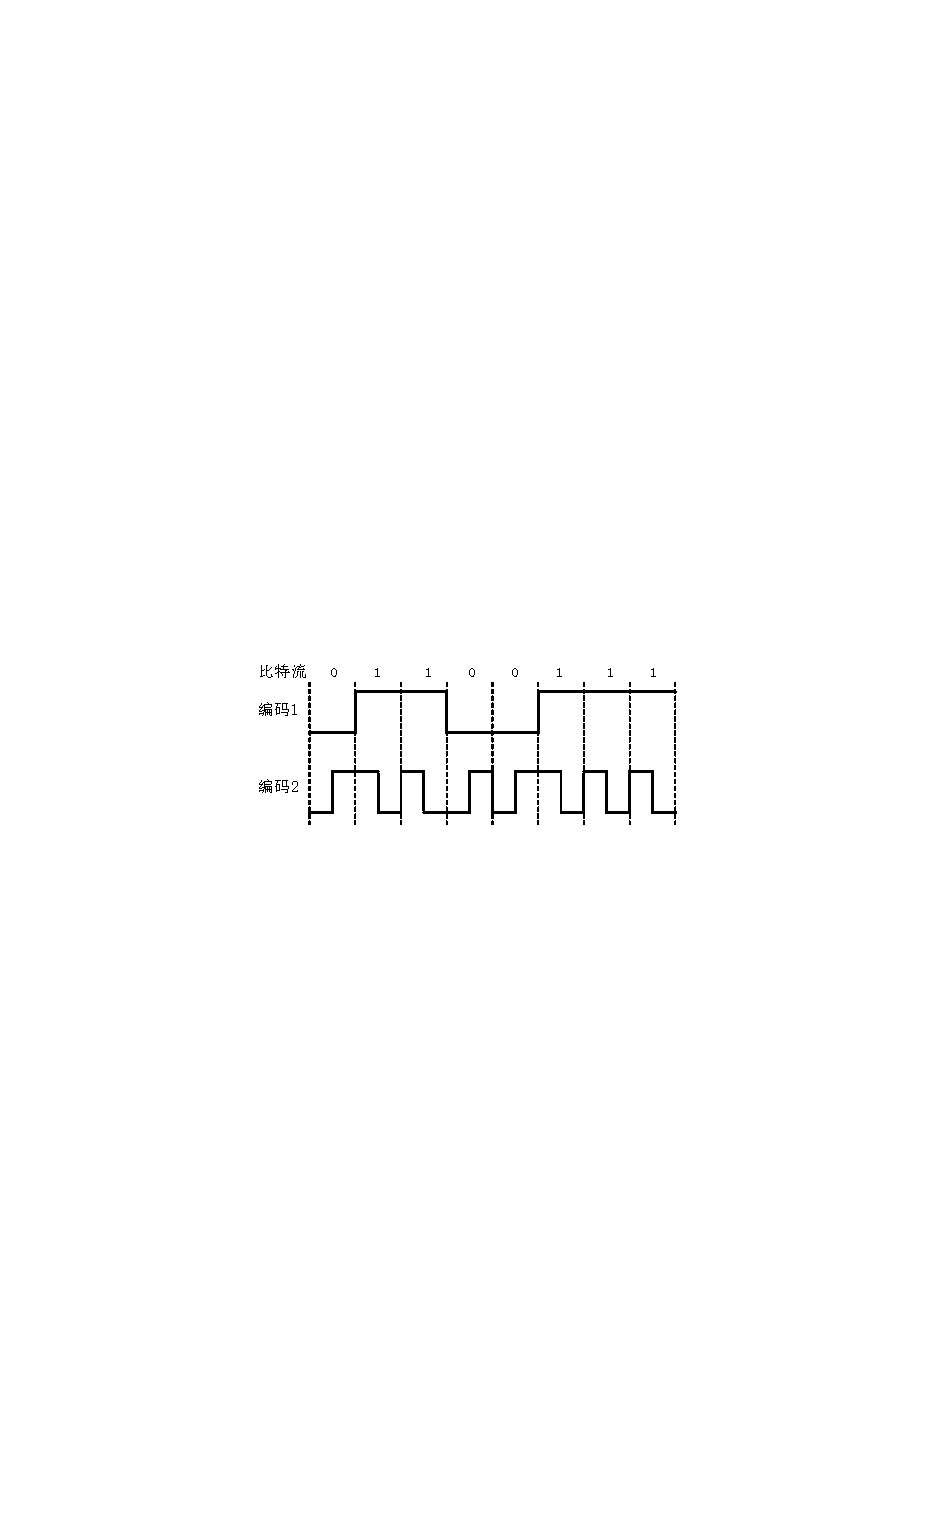
\includegraphics[width=.65\linewidth,height=.4\textheight,keepaspectratio]{../assets/figures/2015-complete-p004-b005.pdf}\end{center}

A．NRZ和曼彻斯特编码　B．NRZ和差分曼彻斯特编码　C．NRZI和曼彻斯特编码　D．NRZI和差分曼彻斯特编码


35．主机甲通过128kbps卫星链路，采用滑动窗口协议向主机乙发送数据，链路单向传播延迟为250ms，帧长为1000字节。不考虑确认帧的开销，为使链路利用率不小于80\%，帧序号的比特数至少是\_\_\_\_\_\_。A．3　B．4　C．7　D．8


36．下列关于 CSMA/CD 协议的叙述中，错误的是\_\_\_\_\_\_。A．边发送数据帧，边检测是否发生冲突　B．适用于无线网络，以实现无线链路共享　C．需要根据网络跨距和数据传输速率限定最小帧长　D．当信号传播延迟趋近0时，信道利用率趋近100\%


37．下列关于交换机的叙述中，正确的是\_\_\_\_\_\_。A．以太网交换机本质上是一种多端口网桥　B．通过交换机互连的一组工作站构成一个冲突域　C．交换机每个端口所连网络构成一个独立的广播域　D．以太网交换机可实现采用不同网络层协议的网络互联


38．某路由器的路由表如下表所示：


\begin{center}\begin{adjustbox}{max width=\linewidth}\begin{tabular}{|>{\raggedright\arraybackslash}p{\dimexpr(\linewidth-6\tabcolsep-4\arrayrulewidth)/3\relax}|>{\raggedright\arraybackslash}p{\dimexpr(\linewidth-6\tabcolsep-4\arrayrulewidth)/3\relax}|>{\raggedright\arraybackslash}p{\dimexpr(\linewidth-6\tabcolsep-4\arrayrulewidth)/3\relax}|}\hline
目的网络 & 下一跳 & 接口\\\hline
169.\allowbreak{}96.\allowbreak{}40.\allowbreak{}0/\allowbreak{}23 & 176.\allowbreak{}1.\allowbreak{}1.\allowbreak{}1 & S1\\\hline\end{tabular}\end{adjustbox}\end{center}

\begin{center}\begin{adjustbox}{max width=\linewidth}\begin{tabular}{|>{\raggedright\arraybackslash}p{\dimexpr(\linewidth-6\tabcolsep-4\arrayrulewidth)/3\relax}|>{\raggedright\arraybackslash}p{\dimexpr(\linewidth-6\tabcolsep-4\arrayrulewidth)/3\relax}|>{\raggedright\arraybackslash}p{\dimexpr(\linewidth-6\tabcolsep-4\arrayrulewidth)/3\relax}|}\hline
169.\allowbreak{}96.\allowbreak{}40.\allowbreak{}0/\allowbreak{}25 & 176.\allowbreak{}2.\allowbreak{}2.\allowbreak{}2 & S2\\\hline
169.\allowbreak{}96.\allowbreak{}40.\allowbreak{}0/\allowbreak{}27 & 176.\allowbreak{}3.\allowbreak{}3.\allowbreak{}3 & S3\\\hline
0.\allowbreak{}0.\allowbreak{}0.\allowbreak{}0/\allowbreak{}0 & 176.\allowbreak{}4.\allowbreak{}4.\allowbreak{}4 & S4\\\hline\end{tabular}\end{adjustbox}\end{center}

38．（续）若路由器收到一个目的地址为169.96.40.5的 IP 分组，则转发该 IP 分组的接口是\_\_\_\_\_\_。A．S1　B．S2　C．S3　D．S4


39．主机甲和主机乙新建一个 TCP 连接，甲的拥塞控制初始阈值为32KB，甲向乙始终以 MSS=1KB 大小的段发送数据，并一直有数据发送；乙为该连接分配16KB接收缓存，并对每个数据段进行确认，忽略段传输延迟。若乙收到的数据全部存入缓存，不被取走，则甲从连接建立成功时刻起，未发送超时的情况下，经过4个 RTT 后，甲的发送窗口是\_\_\_\_\_\_。A．1KB　B．8KB　C．16KB　D．32KB


40．某浏览器发出的 HTTP 请求报文如下：


\begin{Verbatim}[breaklines,breakanywhere,fontsize=\small]
GET /index.html HTTP/1.1
Host: www.test.edu.cn
Connection: Close
Cookie: 123456
\end{Verbatim}

下列叙述中，错误的是\_\_\_\_\_\_。A．该浏览器请求浏览 index.html　B．Index.html 存放在 www.test.edu.cn 上　C．该浏览器请求使用持续连接　D．该浏览器曾经浏览过 www.test.edu.cn


\subsection*{二、综合应用题：第41～47小题，共70分。}

41．（15分）用单链表保存 \(\displaystyle m\) 个整数，结点的结构为：[data][link]，且 \(\displaystyle |data|\le n\)（\(\displaystyle n\) 为正整数）。现要求设计一个时间复杂度尽可能高效的算法，对于链表中 data 的绝对值相等的结点，仅保留第一次出现的结点而删除其余绝对值相等的结点。例如，若给定的单链表 head 如下：


\begin{center}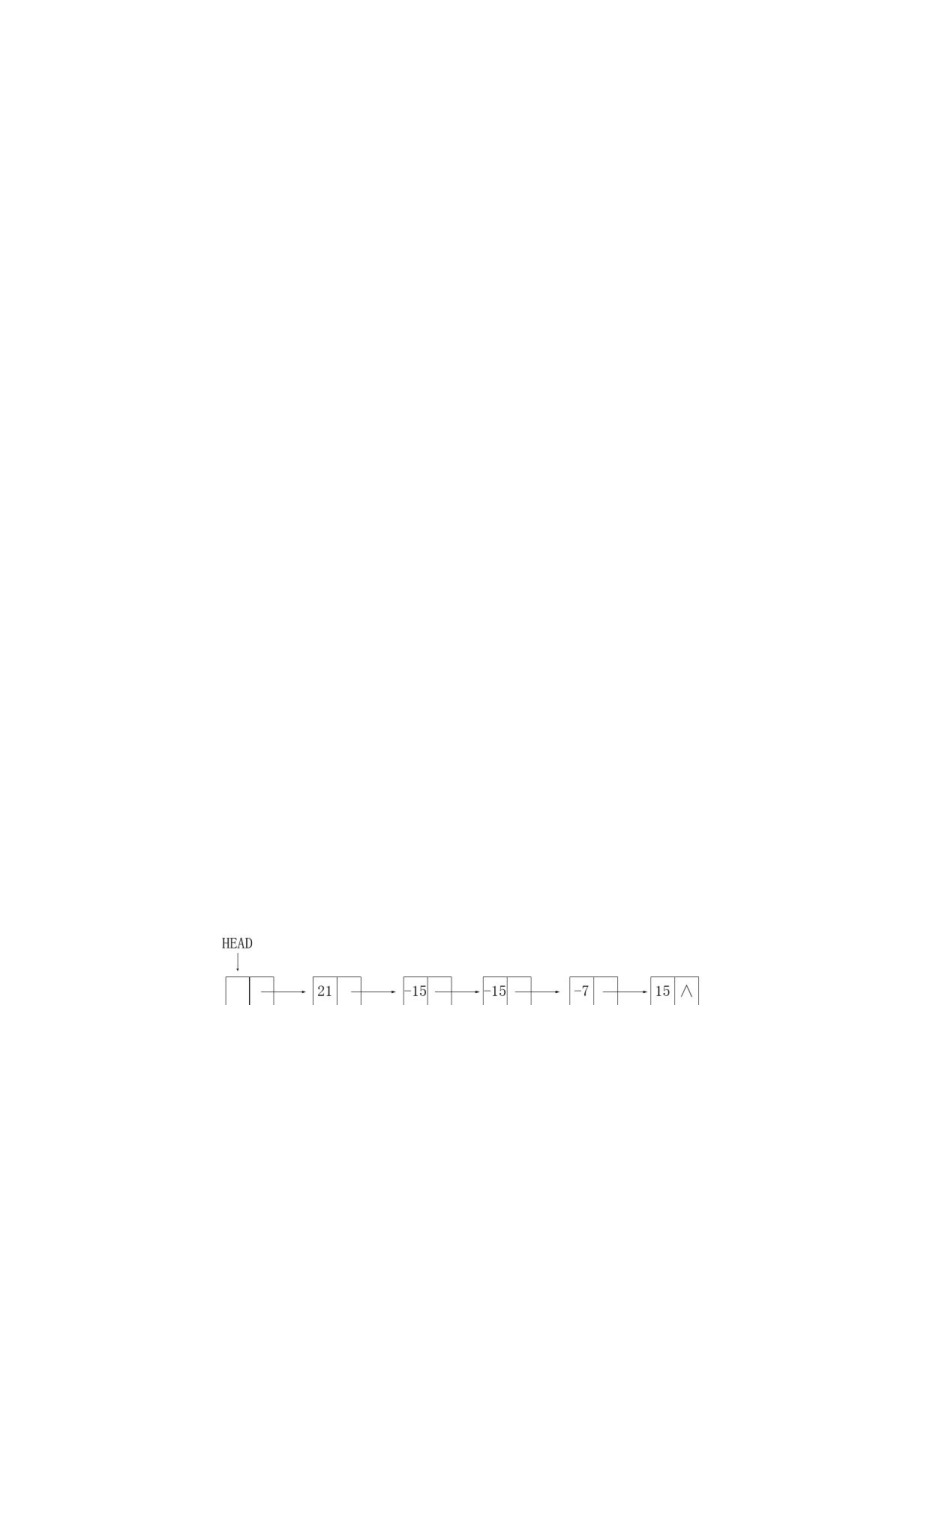
\includegraphics[width=.65\linewidth,height=.4\textheight,keepaspectratio]{../assets/figures/2015-complete-p005-b008.pdf}\end{center}

则删除结点后的 head 为：


\begin{center}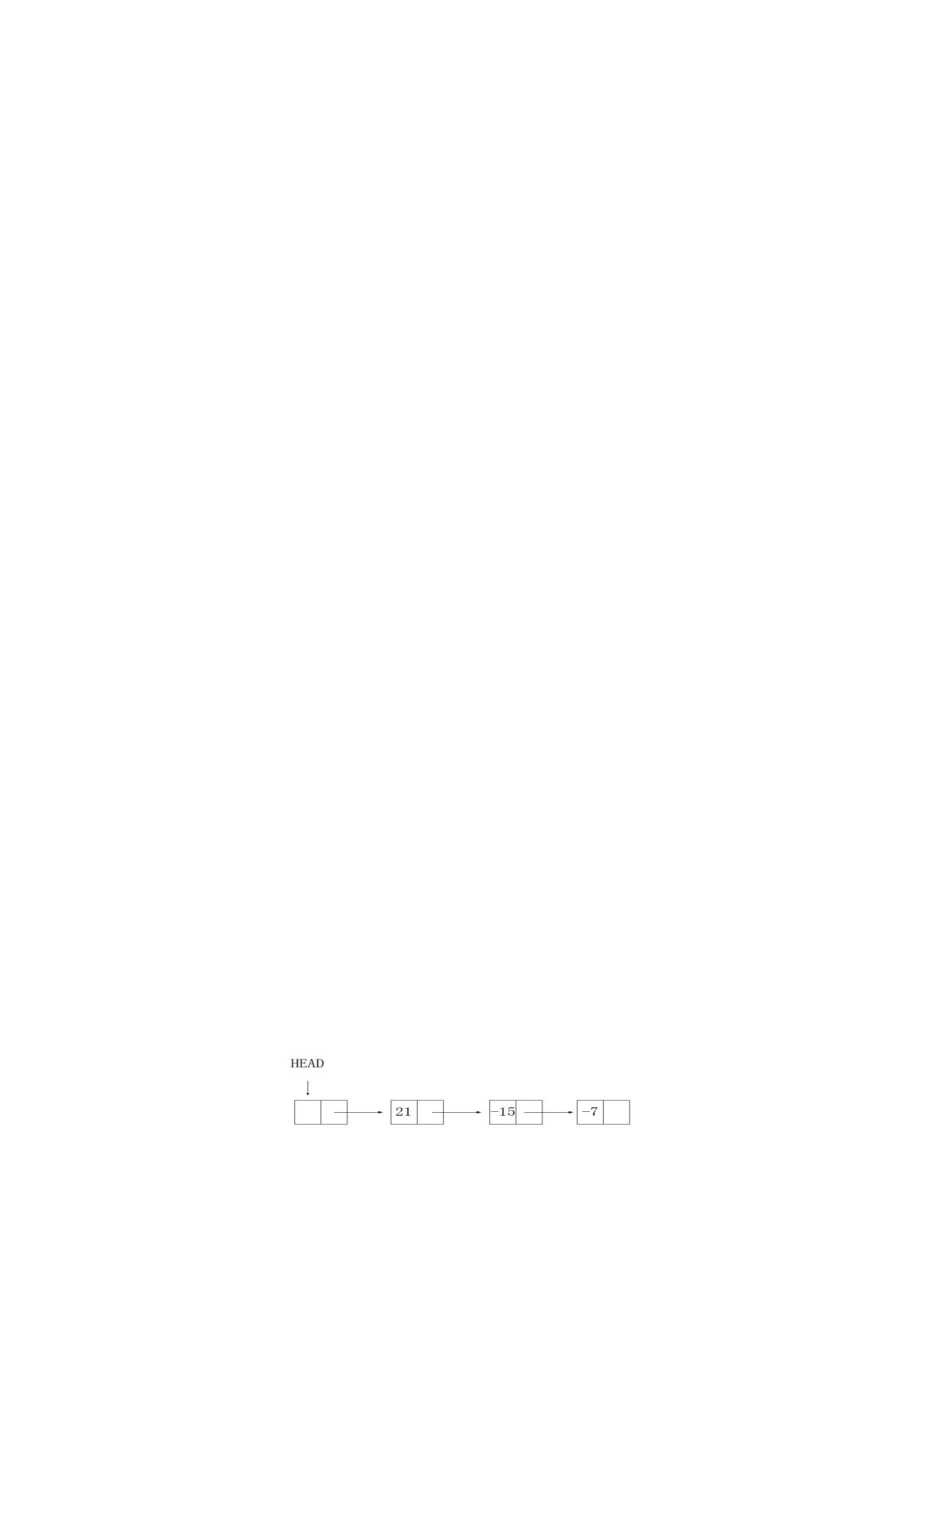
\includegraphics[width=.65\linewidth,height=.4\textheight,keepaspectratio]{../assets/figures/2015-complete-p005-b010.pdf}\end{center}

要求：1）给出算法的基本设计思想。2）使用 C 或 C++语言，给出单链表结点的数据类型定义。3）根据设计思想，采用 C 或 C++语言描述算法，关键之处给出注释。4）说明你所设计算法的时间复杂度和空间复杂度。


42．（8分）已知含有5个顶点的图 \(\displaystyle G\) 如下图所示。


\begin{center}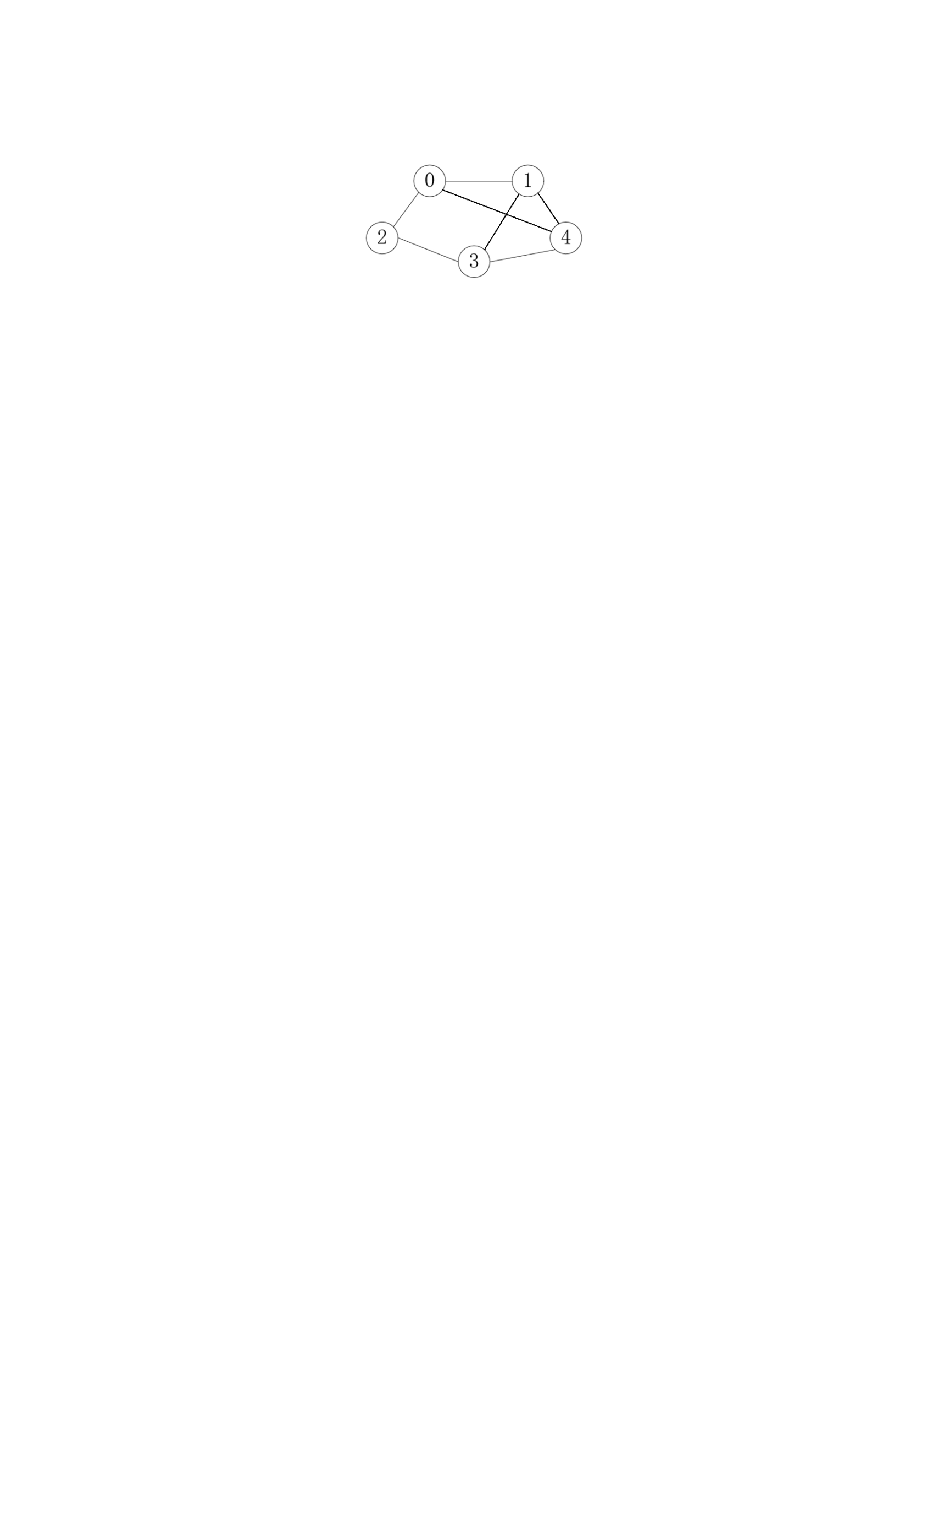
\includegraphics[width=.65\linewidth,height=.4\textheight,keepaspectratio]{../assets/figures/2015-complete-p006-b000.pdf}\end{center}

请回答下列问题：1）写出图 \(\displaystyle G\) 的邻接矩阵 \(\displaystyle A\)（行、列下标从0开始）。2）求 \(\displaystyle A^2\)，矩阵 \(\displaystyle A^2\) 中位于0行3列元素值的含义是什么？3）若已知具有 \(\displaystyle n\)（\(\displaystyle n\ge2\)）个顶点的图的邻接矩阵为 \(\displaystyle B\)，则 \(\displaystyle B^m\)（\(\displaystyle 2\le m\le n\)）中非零元素的含义是什么？


43．（13分）某16位计算机的主存按字节编码，存取单位为16位；采用16位定长指令字格式；CPU采用单总线结构，主要部分如下图所示。图中 R0～R3 为通用寄存器；T 为暂存器；SR 为移位寄存器，可实现直送（mov）、左移一位（left）和右移一位（right）3种操作，控制信号为 SRop，SR 的输出由信号 SRout 控制；ALU 可实现直送 A（mova）、A 加 B（add）、A 减 B（sub）、A 与 B（and）、A 或 B（or）、非 A（not）、A 加1（inc）7种操作，控制信号为 ALUop。


\begin{center}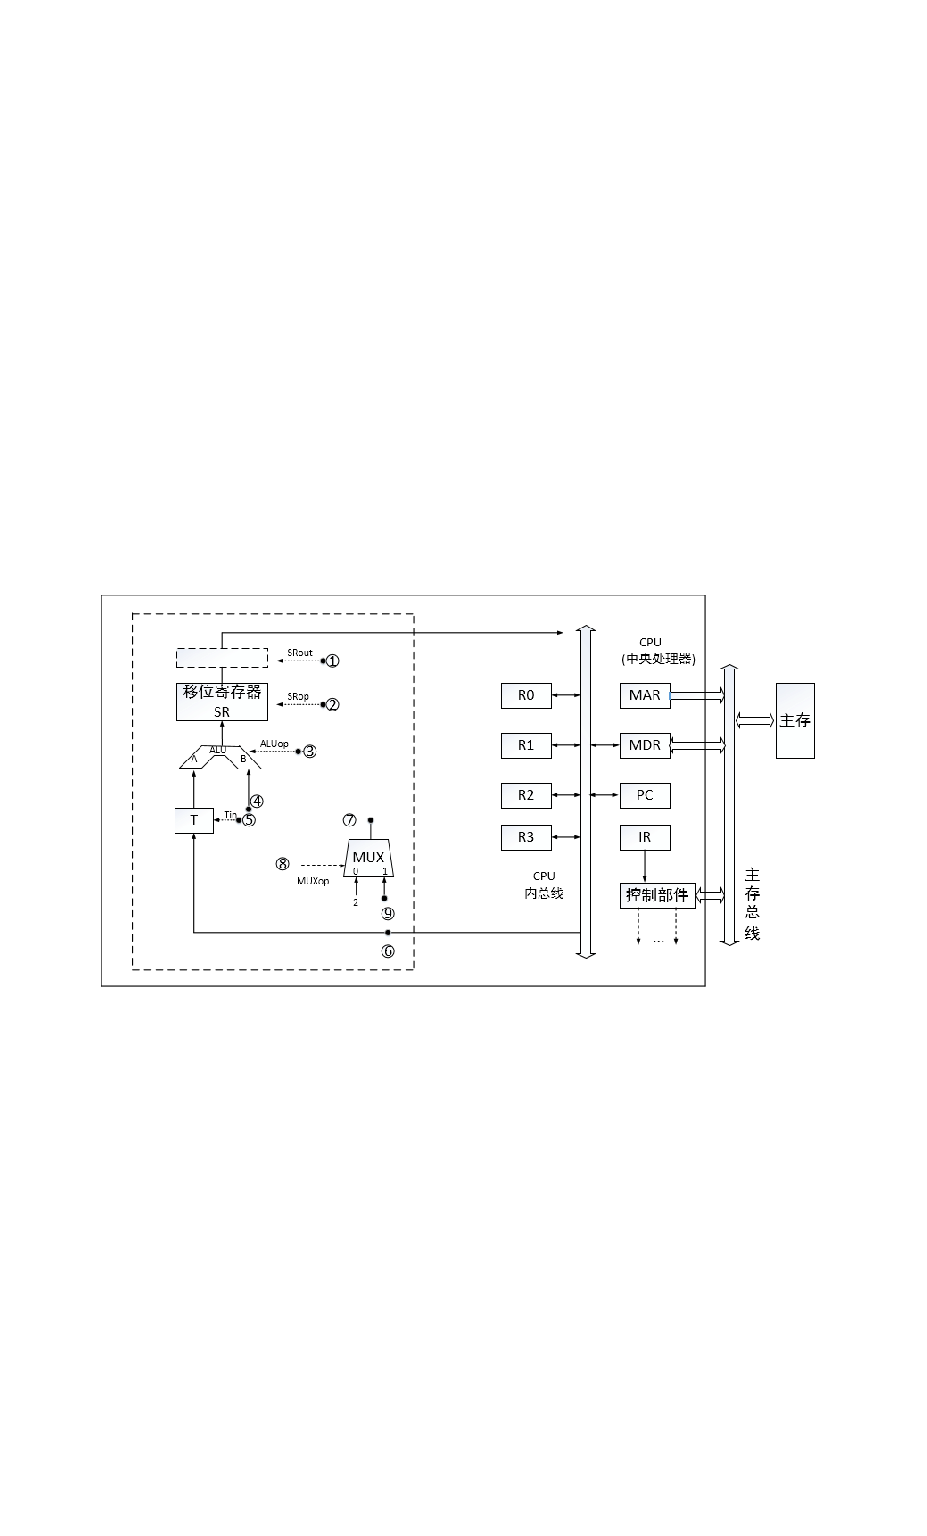
\includegraphics[width=.65\linewidth,height=.4\textheight,keepaspectratio]{../assets/figures/2015-complete-p006-b003.pdf}\end{center}

请回答下列问题。1）图中哪些寄存器是程序员可见的？为何要设置暂存器 T？2）控制信号 ALUop 和 SRop 的位数至少各是多少？3）控制信号 SRout 所控制部件的名称或作用是什么？4）端点\textcircled{1}～\textcircled{9}中，哪些端点须连接到控制部件的输出端？5）为完善单总线数据通路，需要在端点\textcircled{1}～\textcircled{9}中相应的端点之间添加必要的连线。写出连线的起点和终点，以正确表示数据的流动方向。6）为什么二路选择器 MUX 的一个输入端是2？


44．（10分）题43中描述的计算机，其部分指令执行过程的控制信号如下图所示。


\begin{center}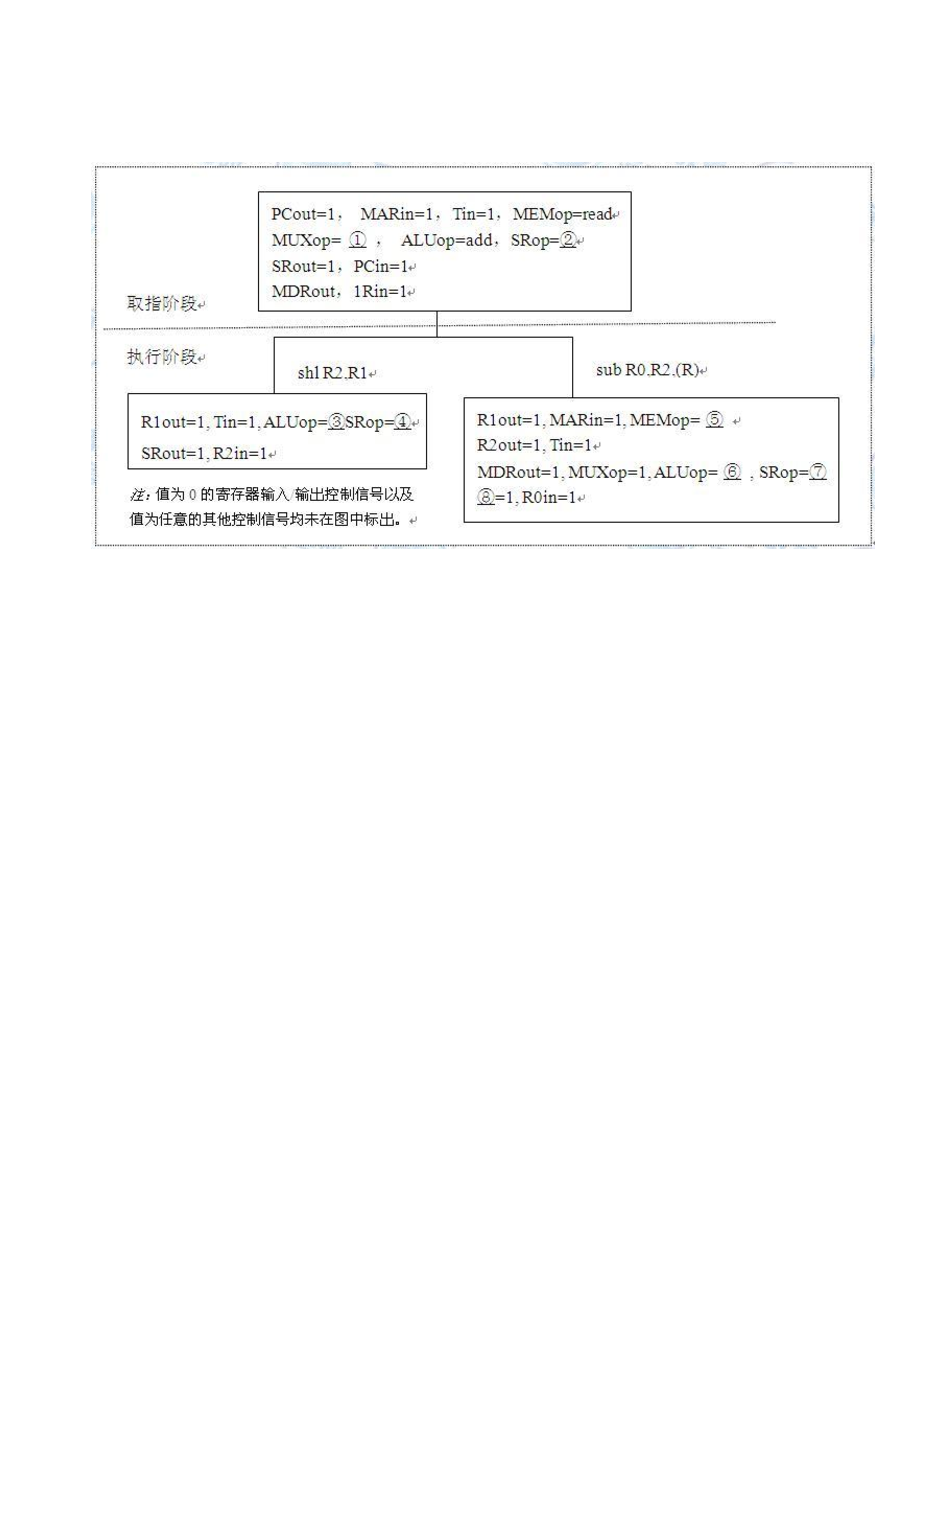
\includegraphics[width=.65\linewidth,height=.4\textheight,keepaspectratio]{../assets/figures/2015-complete-p007-b000.pdf}\end{center}

该机指令格式如下图所示，支持寄存器直接和寄存器间接两种寻址方式，寻址方式位分别为0和1，通用寄存器 R0～R3 的编号分别为0、1、2和3。


\begin{center}\begin{adjustbox}{max width=\linewidth}\begin{tabular}{|>{\raggedright\arraybackslash}p{\dimexpr(\linewidth-14\tabcolsep-8\arrayrulewidth)/7\relax}|>{\raggedright\arraybackslash}p{\dimexpr(\linewidth-14\tabcolsep-8\arrayrulewidth)/7\relax}|>{\raggedright\arraybackslash}p{\dimexpr(\linewidth-14\tabcolsep-8\arrayrulewidth)/7\relax}|>{\raggedright\arraybackslash}p{\dimexpr(\linewidth-14\tabcolsep-8\arrayrulewidth)/7\relax}|>{\raggedright\arraybackslash}p{\dimexpr(\linewidth-14\tabcolsep-8\arrayrulewidth)/7\relax}|>{\raggedright\arraybackslash}p{\dimexpr(\linewidth-14\tabcolsep-8\arrayrulewidth)/7\relax}|>{\raggedright\arraybackslash}p{\dimexpr(\linewidth-14\tabcolsep-8\arrayrulewidth)/7\relax}|}\hline
指令操作码 & 目的操作数 & 目的操作数 & 源操作数1 & 源操作数1 & 源操作数2 & 源操作数2\\\hline
OP & Md & Rd & Ms1 & Rs1 & Ms2 & Rs2\\\hline\end{tabular}\end{adjustbox}\end{center}

题图b：指令格式。其中 Md、Ms1、Ms2 为寻址方式位，Rd、Rs1、Rs2 为寄存器编号。三地址指令：源操作数1 OP 源操作数2→目的操作数地址；二地址指令（末3位均为0）：OP 源操作数1→目的操作数地址；单地址指令（末6位均为0）：OP 目的操作数→目的操作数地址。


请回答下列问题。1）该机的指令系统最多可定义多少条指令？2）假定 inc、shl 和 sub 指令的操作码分别为01H、02H和03H，则以下指令对应的机器代码各是什么？


\begin{Verbatim}[breaklines,breakanywhere,fontsize=\small]
① inc R1             ; R1 + 1 → R1
② shl R2,R1          ; (R1) << 1 → R2
③ sub R3,(R1),R2     ; ((R1)) - (R2) → R3
\end{Verbatim}

3）假设寄存器 X 的输入和输出控制信号分别为 Xin 和 Xout，其值为1表示有效，为0表示无效（例如，PCout=1表示 PC 内容送总线）；存储器控制信号为 MEMop，用于控制存储器的读（read）和写（write）操作。写出题图a中标号\textcircled{1}～\textcircled{8}处的控制信号或控制信号的取值。4）指令“sub R1,R3,(R2)”和“inc R1”的执行阶段至少各需要多少个时钟周期？


45．（9分）有 A、B 两人通过信箱进行辩论，每个人都从自己的信箱中取得对方的问题。将答案和向对方提出的新问题组成一个邮件放入对方的邮箱中。假设 A 的信箱最多放 \(\displaystyle M\) 个邮件，B 的信箱最多放 \(\displaystyle N\) 个邮件。初始时 A 的信箱中有 \(\displaystyle x\) 个邮件（\(\displaystyle 0<x<M\)），B 的信箱中有 \(\displaystyle y\) 个（\(\displaystyle 0<y<N\)）。辩论者每取出一个邮件，邮件数减1。A 和 B 两人的操作过程描述如下：


\begin{Verbatim}[breaklines,breakanywhere,fontsize=\small]
CoBegin
\end{Verbatim}

\begin{Verbatim}[breaklines,breakanywhere,fontsize=\small]
A{
  while(TRUE){
    从A的信箱中取出一个邮件；
    回答问题并提出一个新问题；
    将新邮件放入B的信箱；
  }
}
B{
  while(TRUE){
    从B的信箱中取出一个邮件；
    回答问题并提出一个新问题；
    将新邮件放入A的信箱；
  }
}
CoEnd
\end{Verbatim}

当信箱不为空时，辩论者才能从信箱中取邮件，否则等待。当信箱不满时，辩论者才能将新邮件放入信箱，否则等待。请添加必要的信号量和 P、V（或 wait、signal）操作，以实现上述过程的同步。要求写出完整过程，并说明信号量的含义和初值。


46．（6分）某计算机系统按字节编址，采用二级页表的分页存储管理方式，虚拟地址格式如下所示：


\begin{center}\begin{adjustbox}{max width=\linewidth}\begin{tabular}{|>{\raggedright\arraybackslash}p{\dimexpr(\linewidth-6\tabcolsep-4\arrayrulewidth)/3\relax}|>{\raggedright\arraybackslash}p{\dimexpr(\linewidth-6\tabcolsep-4\arrayrulewidth)/3\relax}|>{\raggedright\arraybackslash}p{\dimexpr(\linewidth-6\tabcolsep-4\arrayrulewidth)/3\relax}|}\hline
10位 & 10位 & 12位\\\hline
页目录号 & 页表索引 & 页内偏移量\\\hline\end{tabular}\end{adjustbox}\end{center}

请回答下列问题。1）页和页框的大小各为多少字节？进程的虚拟地址空间大小为多少页？2）假定页目录项和页表项均占4个字节，则进程的页目录和页表共占多少页？要求写出计算过程。3）若某指令周期内访问的虚拟地址为0100 0000H和0111 2048H，则进行地址转换时共访问多少个二级页表？要求说明理由。


47．（9分）某网络拓扑如图所示，其中路由器内网接口、DHCP服务器、WWW服务器与主机1均采用静态 IP 地址配置，相关地址信息见图中标注；主机2～主机N通过 DHCP 服务器动态获取 IP 地址等配置信息。


\begin{center}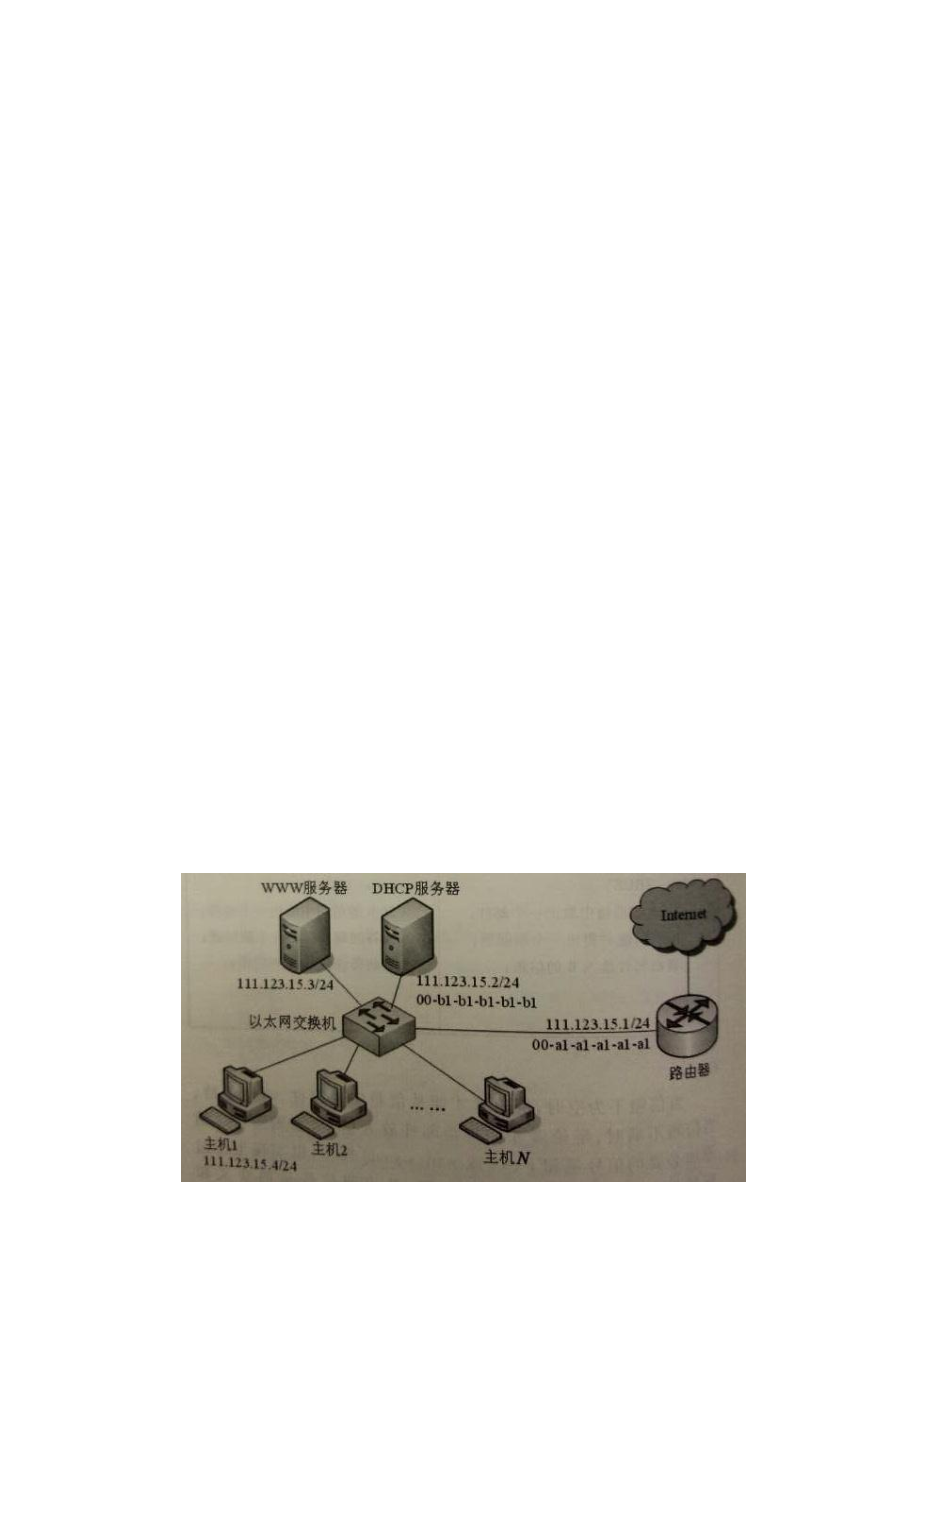
\includegraphics[width=.65\linewidth,height=.4\textheight,keepaspectratio]{../assets/figures/2015-complete-p008-b006.pdf}\end{center}

请回答下列问题。1）DHCP服务器可为主机2～主机N动态分配 IP 地址的最大范围是什么？主机2使用 DHCP 协议获取 IP 地址的过程中，发送的封装 DHCP Discover


2）若主机2的 ARP 表为空，则该主机访问 Internet 时，发出的第一个以太网帧的目的 MAC 地址是什么？封装主机2发往 Internet 的 IP 分组的以太网帧的目的 MAC 地址是什么？


3）若主机1的子网掩码和默认网关分别配置为255.255.255.0和111.123.15.2，则该主机是否能访问 WWW 服务器？是否能访问 Internet？请说明理由。


\subsection*{2015年计算机学科专业基础综合试题参考答案}

\subsection*{一、单项选择题}

1．A　2．B　3．D　4．D　5．D　6．C　7．A　8．C　9．C　10．C　11．A　12．A　13．B　14．D　15．C　16．B　17．B　18．D　19．C　20．B　21．B　22．D　23．B　24．C　25．D　26．B　27．A　28．A　29．B　30．C　31．C　32．C　33．D　34．A　35．B　36．B　37．A　38．C　39．A　40．C


\subsection*{二、综合应用题}

41．解答：1）算法的基本设计思想。算法的核心思想是用空间换时间。使用辅助数组记录链表中已出现的数值，从而只需对链表进行一趟扫描。因为 \(\displaystyle |data|\le n\)，故辅助数组 q 的大小为 \(\displaystyle n+1\)，各元素的初值均为0。依次扫描链表中的各结点，同时检查 q[|data|] 的值，如果为0，则保留该结点，并令 q[|data|]=1；否则，将该结点从链表中删除。


2）使用 C 语言描述的单链表结点的数据类型定义：


\begin{Verbatim}[breaklines,breakanywhere,fontsize=\small]
typedef struct node {
  int data;
  struct node *link;
}NODE;
Typedef NODE *PNODE;
\end{Verbatim}

3）算法实现：


\begin{Verbatim}[breaklines,breakanywhere,fontsize=\small]
void func (PNODE h,int n)
{  PNODE p=h,r;
   int *q,m;
   q=(int *)malloc(sizeof(int)*(n+1));//申请n+1个位置的辅助空间
   for(int i=0;i<n+1;i++)   //数组元素初值置0
      *(q+i)=0;
   while(p->link!=NULL)
   {  m=p->link->data>0? p->link->data:-p->link->data;
      if(*(q+m)==0)       //判断该结点的data是否已出现过
      {  *(q+m)=1;          //首次出现
         p=p->link;        //保留
      }
      else                //重复出现
      {  r=p->link;        //删除
         p->link=r->link
         free(r);
      }
   }
   free(q);
}
\end{Verbatim}

【评分说明】若考生设计的算法满足题目的功能要求且正确，则酌情给分。


41．（续）4）参考答案所给算法的时间复杂度为 \(\displaystyle O(m)\)，空间复杂度为 \(\displaystyle O(n)\)。


【评分说明】若考生所估计的时间复杂度和空间复杂度与考生实现的算法一致，可给分。


42．解答：1）图 \(\displaystyle G\) 的邻接矩阵 \(\displaystyle A\) 如下：


\[\fitmath{\displaystyle A=\begin{bmatrix}0&1&1&0&1\\1&0&0&1&1\\1&0&0&1&0\\0&1&1&0&1\\1&1&0&1&0\end{bmatrix}}\]

2）\(\displaystyle A^2\) 如下：


\[\fitmath{\displaystyle A^2=\begin{bmatrix}3&1&0&3&1\\1&3&2&1&2\\0&2&2&0&2\\3&1&0&3&1\\1&2&2&1&3\end{bmatrix}}\]

0行3列的元素值3表示从顶点0到顶点3之间长度为2的路径共有3条。


3）\(\displaystyle B^m\)（\(\displaystyle 2\le m\le n\)）中位于 i 行 j 列（\(\displaystyle 0\le i,\allowbreak j\le n-1\)）的非零元素的含义是：图中从顶点 i 到顶点 j 长度为 m 的路径条数。


43．解答：1）程序员可见寄存器为通用寄存器（R0～R3）和 PC。因为采用了单总线结构，因此，若无暂存器 T，则 ALU 的 A、B 端口会同时获得两个相同的数据，使数据通路不能正常工作。


【评分说明】回答通用寄存器（R0～R3），给分；回答 PC，给分；部分正确，酌情给分。设置暂存器 T 的原因若回答用于暂时存放端口 A 的数据，则给分，其他答案，酌情给分。


2）ALU 共有7种操作，故其操作控制信号 ALUop 至少需要3位；移位寄存器有3种操作，其操作控制信号 SRop 至少需要2位。


3）信号 SRout 所控制的部件是一个三态门，用于控制移位器与总线之间数据通路的连接与断开。


【评分说明】只要回答出三态门或者控制连接/断开，即给分。


4）端口\textcircled{1}、\textcircled{2}、\textcircled{3}、\textcircled{5}、\textcircled{8}须连接到控制部件输出端。


【评分说明】答案包含\textcircled{4}、\textcircled{6}、\textcircled{7}、\textcircled{9}中任意一个，不给分；答案不全酌情给分。


5）连线1，\textcircled{6}→\textcircled{9}；连线2，\textcircled{7}→\textcircled{4}。


【评分说明】回答除上述连线以外的其他连线，酌情给分。


6）因为每条指令的长度为16位，按字节编址，所以每条指令占用2个内存单元，顺序执行时，下条指令地址为（PC）+2。MUX 的一个输入端为2，可便于执行（PC）+2操作。


44．解答：1）指令操作码有7位，因此最多可定义 \(\displaystyle 2^7=128\) 条指令。2）各条指令的机器代码分别如下：


44．（续）\textcircled{1}“inc R1”的机器码为：0000001 0 01 0 00 0 00，即0240H。\textcircled{2}“shl R2,R1”的机器码为：0000010 0 10 0 01 0 00，即0488H。\textcircled{3}“sub R3,(R1),R2”的机器码为：0000011 0 11 1 01 0 10，即06EAH。


3）各标号处的控制信号或控制信号取值如下：\textcircled{1}0；\textcircled{2}mov；\textcircled{3}mova；\textcircled{4}left；\textcircled{5}read；\textcircled{6}sub；\textcircled{7}mov；\textcircled{8}Srout。


【评分说明】答对两个给分。


4）指令“sub R1,R3,(R2)”的执行阶段至少包含4个时钟周期；指令“inc R1”的执行阶段至少包含2个时钟周期。


45．解答：


\begin{Verbatim}[breaklines,breakanywhere,fontsize=\small]
semaphore Full_A = x;      // Full_A表示A的信箱中的邮件数量
semaphore Empty_A = M-x;   // Empty_A表示A的信箱中还可存放的邮件数量
semaphore Full_B = y;      // Full_B表示B的信箱中的邮件数量
semaphore Empty_B = N-y;   // Empty_B表示B的信箱中还可存放的邮件数量
semaphore mutex_A = 1;    // mutex_A用于A的信箱互斥
semaphore mutex_B = 1;    // mutex_B用于B的信箱互斥
Cobegin
A{
  while(TRUE){
    P(Full_A);
    P(mutex_A);
    从A的信箱中取出一个邮件;
    V(mutex_A);
    V(Empty_A);
    回答问题并提出一个新问题;
    P(Empty_B);
    P(mutex_B);
    将新邮件放入B的信箱;
    V(mutex_B);
    V(Full_B);
  }
}
B{
  while(TRUE){
    P(Full_B);
    P(mutex_B);
    从B的信箱中取出一个邮件;
    V(mutex_B);
    V(Empty_B);
    回答问题并提出一个新问题;
    P(Empty_A);
    P(mutex_A);
    将新邮件放入A的信箱;
    V(mutex_A);
    V(Full_A);
  }
}
\end{Verbatim}

【评分说明】1）每对信号量的定义及初值正确，给分。2）每个互斥信号量的 P、V 操作使用正确，各给分。3）每个同步信号量的 P、V 操作使用正确，各给分。4）其他答案酌情给分。


46．解答：1）页和页框大小均为4KB。进程的虚拟地址空间大小为 \(\displaystyle 2^{32}/2^{12}=2^{20}\) 页。


2）\(\displaystyle (2^{10}\times4)/2^{12}\)（页目录所占页数）\(\displaystyle +\,(2^{20}\times4)/2^{12}\)（页表所占页数）\(\displaystyle =1025\) 页。


3）需要访问一个二级页表。因为虚拟地址0100 0000H和0111 2048H的最高10位的值都是4，访问的是同一个二级页表。


【评分说明】用其他方法计算，思路和结果正确同样给分。


47．解答：1）DHCP服务器可为主机2～主机N动态分配 IP 地址的最大范围是：111.123.15.5～111.123.15.254；主机2发送的封装 DHCP Discover 报文的 IP 分组的源 IP 地址和目的 IP 地址分别是0.0.0.0和255.255.255.255。


2）主机2发出的第一个以太网帧的目的 MAC 地址是 ff-ff-ff-ff-ff-ff；封装主机2发往 Internet 的 IP 分组的以太网帧的目的 MAC 地址是00-a1-a1-a1-a1-a1。


3）主机1能访问 WWW 服务器，但不能访问 Internet。由于主机1的子网掩码配置正确而默认网关 IP 地址被错误地配置为111.123.15.2（正确 IP 地址是111.123.15.1），所以主机1可以访问在同一个子网内的 WWW 服务器，但当主机1访问 Internet 时，主机1发出的 IP 分组会被路由到错误的默认网关（111.123.15.2），从而无法到达目的主机。

\end{document}
